\documentclass[a4paper,12pt]{article}
\usepackage[utf8]{inputenc}
\usepackage{csquotes}
\usepackage[T1]{fontenc}
\usepackage[polish]{babel}
\usepackage{xcolor}
\usepackage{graphicx}
\usepackage{amsmath}
\usepackage{amssymb}
\usepackage{hyperref}
\usepackage{float}
\usepackage{listings}
\usepackage[backend=biber, style=numeric]{biblatex}

\addbibresource{bibliografia.bib}

\lstset{
  basicstyle=\ttfamily\small,
  columns=flexible,
  keepspaces=true,
  showstringspaces=false,
  escapeinside={(*@}{@*)},
  literate={ą}{{\k{a}}}1
           {ć}{{\'{c}}}1
           {ę}{{\k{e}}}1
           {ł}{{\l{}}}1
           {ń}{{\'{n}}}1
           {ó}{{\'{o}}}1
           {ś}{{\'{s}}}1
           {ź}{{\'{z}}}1
           {ż}{{\.{z}}}1
           {Ą}{{\k{A}}}1
           {Ć}{{\'{C}}}1
           {Ę}{{\k{E}}}1
           {Ł}{{\L{}}}1
           {Ń}{{\'{N}}}1
           {Ó}{{\'{O}}}1
           {Ś}{{\'{S}}}1
           {Ź}{{\'{Z}}}1
           {Ż}{{\.{Z}}}1
           {"}{{\textquotedbl}}1
           {'}{{\textquotesingle}}1
           {`}{{\textasciigrave}}1
           {~}{{\textasciitilde}}1
           {^}{{\textasciicircum}}1
           {_}{{\textunderscore}}1
           {|}{{\textbar}}1
           {\{}{{\textbraceleft}}1
           {\}}{{\textbraceright}}1
           {[}{{[}}1
           {]}{{]}}1,
  language=SQL,
  showspaces=false,
  numbers=left,
  numberstyle=\tiny,
  commentstyle=\color{green!60!black},
  keywordstyle=\color{blue},
  stringstyle=\color{red!80!black},
  breaklines=true, 
  frame=single,
  captionpos=b 
}

\title{6. sprawozdanie z laboratorium Hurtownie Danych}
\author{Mikołaj Kubś, 272662}
\date{\today}

\begin{document}

\maketitle

\section{Zad. 1. Modyfikacja wymiarów i tabeli faktów}

Bazując na kostce utworzonej przy realizacji listy 4, należy:

\subsection{Podpunkt a}

Zmodyfikować definicję wymiarów tak, aby:

\begin{enumerate}
  \item W wymiarach CUSTOMER i SALESPERSON nie można było korzystać z atrybutów FirstName oraz LastName. W zamian dodać atrybut Names\\
        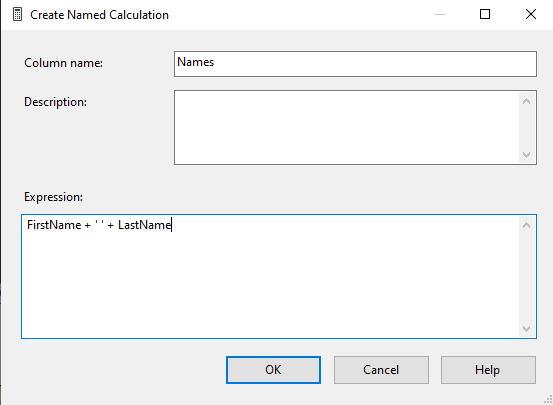
\includegraphics[width=0.6\textwidth]{images/1a1.png}

  \item W wymiarze SALESPERSON pojawiła się hierarchia Group - CountryRegionCode - Names\\
        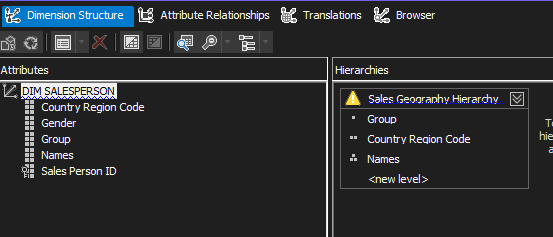
\includegraphics[width=0.6\textwidth]{images/1a2.png}

  \item W wymiarze CUSTOMER pojawiła się hierarchia Group - CountryRegionCode - Names\\
        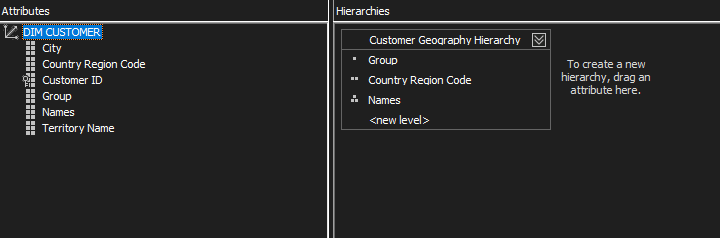
\includegraphics[width=0.6\textwidth]{images/1a3.png}

  \item W wymiarze PRODUCT pojawiła się hierarchia CategoryName - SubCategoryName - Name\\
        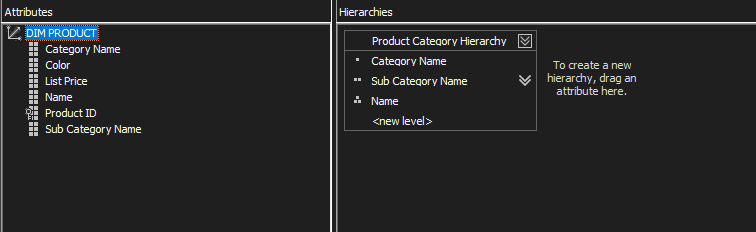
\includegraphics[width=0.6\textwidth]{images/1a4.png}

  \item W wymiarze TIME pojawiła się hierarchia Rok - Kwartał - Miesiąc - Dzień miesiąca\\
        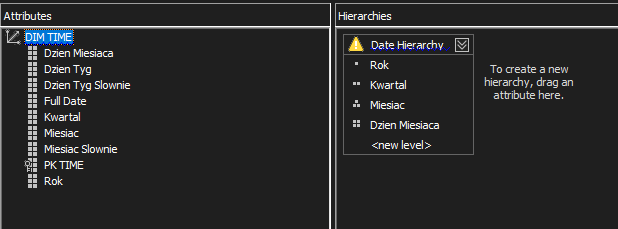
\includegraphics[width=0.6\textwidth]{images/1a5.png}
\end{enumerate}

\subsection{Podpunkt b}

Dla każdego atrybutu kluczowego wymiaru, którego wartościami są liczby całkowite,
zmodyfikować właściwości (Properties). Zmodyfikować parametr NameColumn, tak
aby nazwy kolejnych elementów wymiaru nie były liczbami. (Przykładowo dla wymiaru dotyczącego Produktu można wykorzystać atrybut Name).

\begin{figure}[H]
  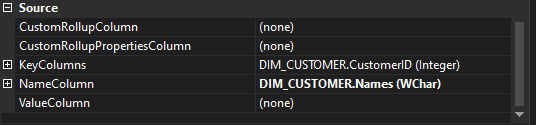
\includegraphics[width=0.6\textwidth]{images/1b_salesperson.png}
  \caption{Widok Properties dla DIM\_Salesperson}
\end{figure}

\begin{figure}[H]
  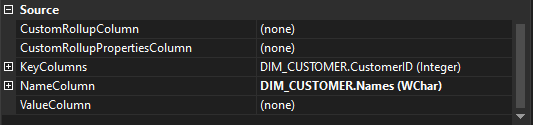
\includegraphics[width=0.6\textwidth]{images/1b_customer.png}
  \caption{Widok Properties dla DIM\_Customer}
\end{figure}

\begin{figure}[H]
  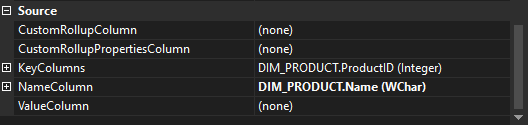
\includegraphics[width=0.6\textwidth]{images/1b_product.png}
  \caption{Widok Properties dla DIM\_Product}
\end{figure}

\begin{figure}[H]
  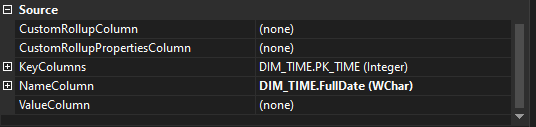
\includegraphics[width=0.6\textwidth]{images/1b_time.png}
  \caption{Widok Properties dla DIM\_Time}
\end{figure}

\subsection{Podpunkt c}

Utworzyć nowe miary, które będą odzwierciedlać:

\begin{itemize}
  \item Liczbę różnych klientów (aggregatedFunction: distinct count)
  \item Liczbę różnych produktów
  \item Maksymalną wartość rabatu (aggregatedFunction: max)
  \item Maksymalną liczbę zamówionych produktów
  \item Liczbę różnych sprzedawców realizujących zamówienia
\end{itemize}

\begin{figure}[H]
  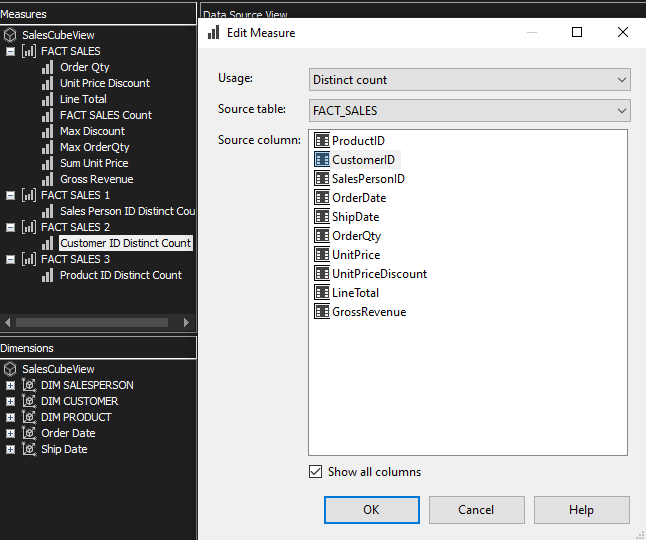
\includegraphics[width=0.6\textwidth]{images/1c.png}
  \caption{Miara dotycząca liczby różnych klientów}
\end{figure}

\subsection{Podpunkt d}

Wdrożyć i przeprocesować kostkę.

\begin{figure}[H]
  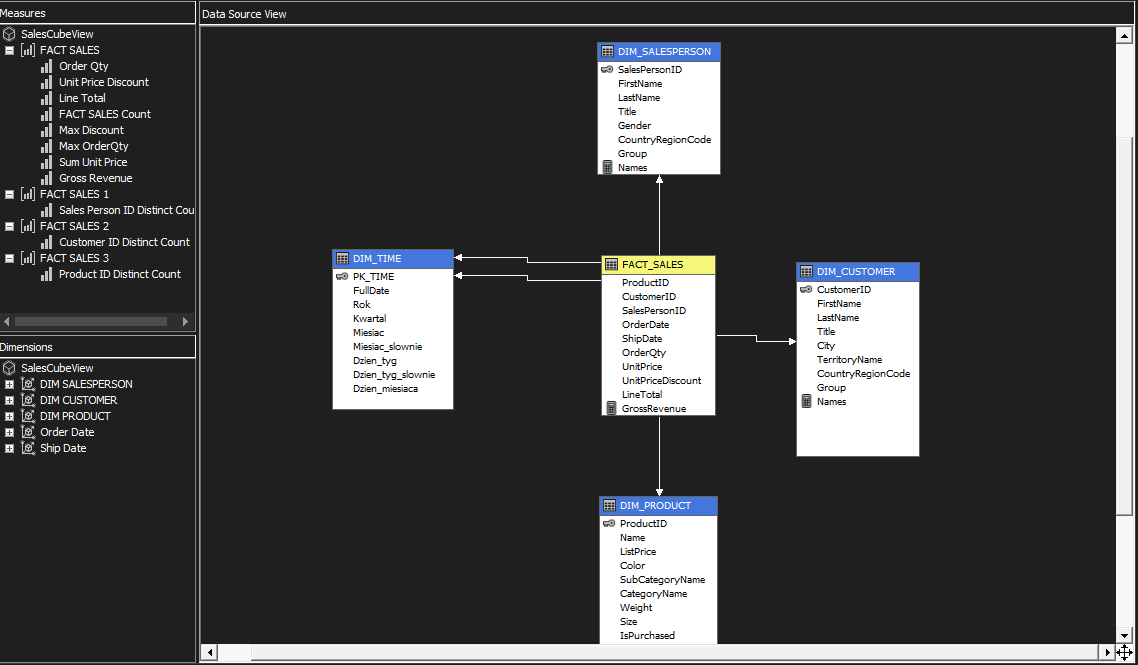
\includegraphics[width=0.6\textwidth]{images/1d.png}
  \caption{Widok przeprocesowanej kostki}
\end{figure}

\section{Zad. 2. Przegląd danych i tworzenie zestawień}

Przy użyciu zakładki Browser:

\subsection{Podpunkt a}

Sprawdzić, czy dane zapisane w kostce zgadzają się z danymi zapisanymi w tabelach, przeciągając za pomocą myszy:
\begin{itemize}
  \item atrybuty wymiarów w region wierszy
  \item miary w część centralną widoku
\end{itemize}

\begin{figure}[H]
  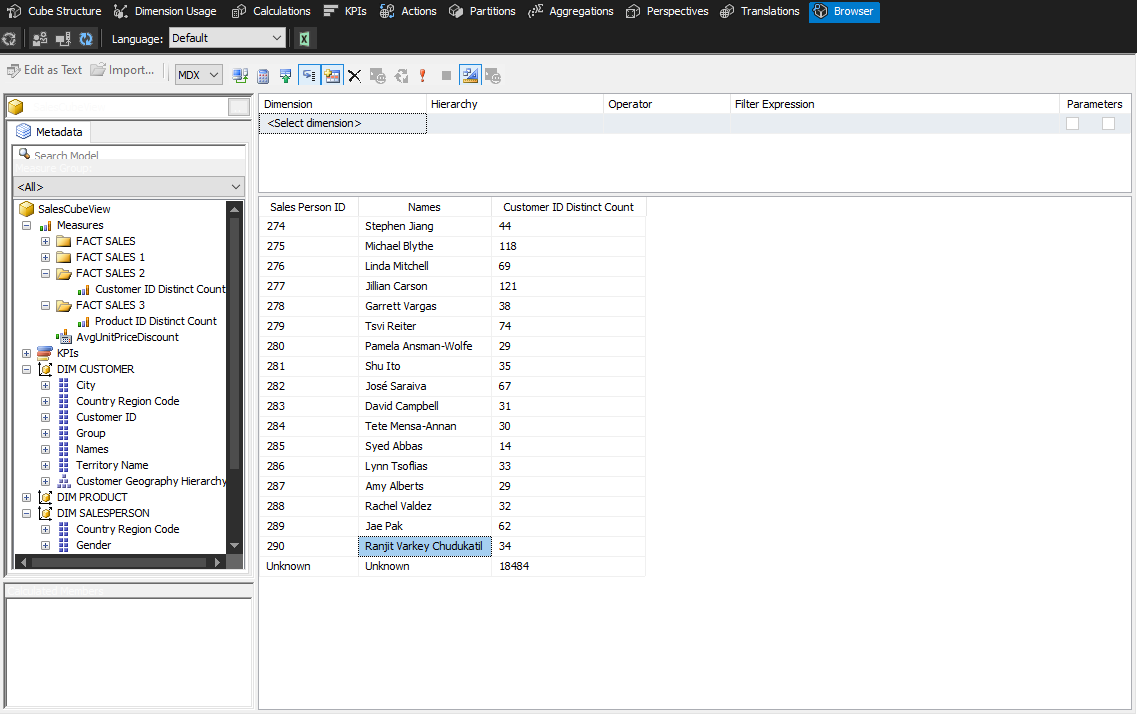
\includegraphics[width=0.6\textwidth]{images/2a.png}
  \caption{Widok przykładowej kwerendy w Browser}
\end{figure}

\subsection{Podpunkt b}

Przetestować możliwości przeglądarki (Browser) - operator wyboru danych (Operator), wyrażenia filtrujące dane (Filter Expression) itp.

\begin{figure}[H]
  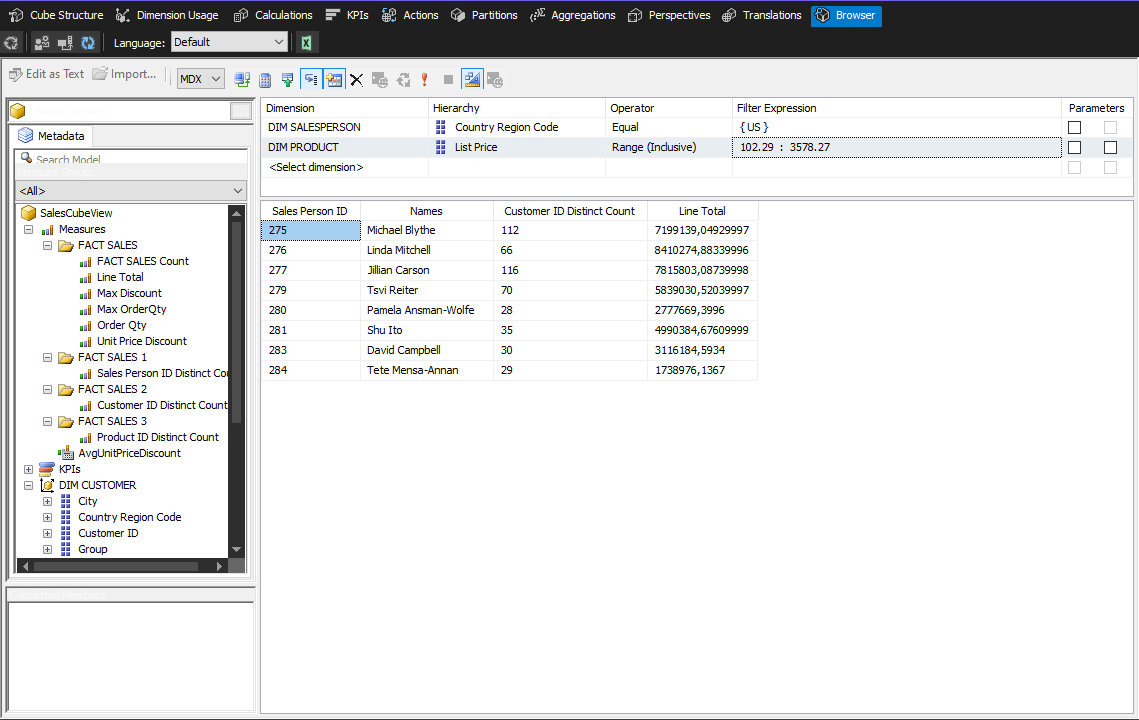
\includegraphics[width=0.6\textwidth]{images/2b.png}
  \caption{Widok przykładowej kwerendy z dwoma różnymi rodzajami filtrów (Operator i Filter Expression)}
\end{figure}

\subsection{Podpunkt c}

Przygotować przykładowe tabele i wykresy przestawne oraz zinterpretować uzyskane
wyniki (proszę zapisać wnioski!)

\subsubsection{Rowery}

\begin{figure}[H]
  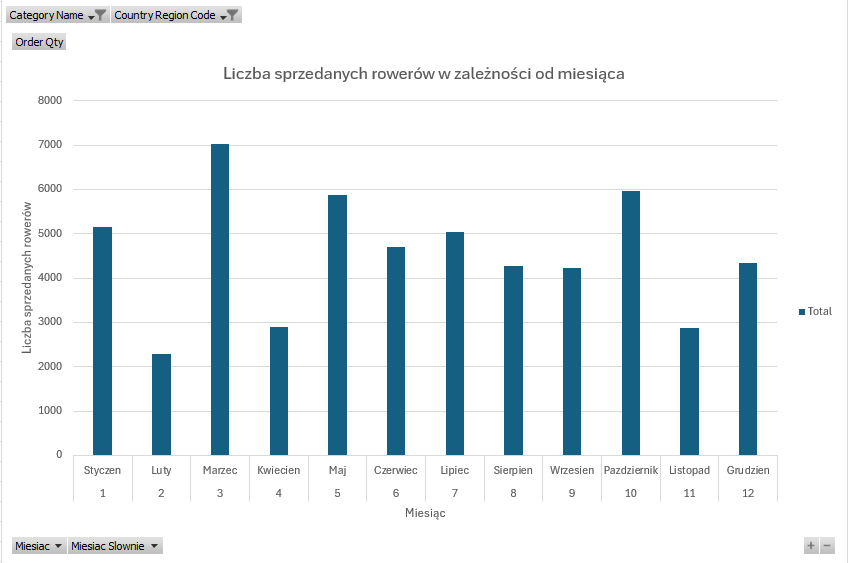
\includegraphics[width=0.6\textwidth]{images/bike_sales.png}
  \caption{Wykres}
\end{figure}

\subsubsection{Rowery}

\begin{figure}[H]
  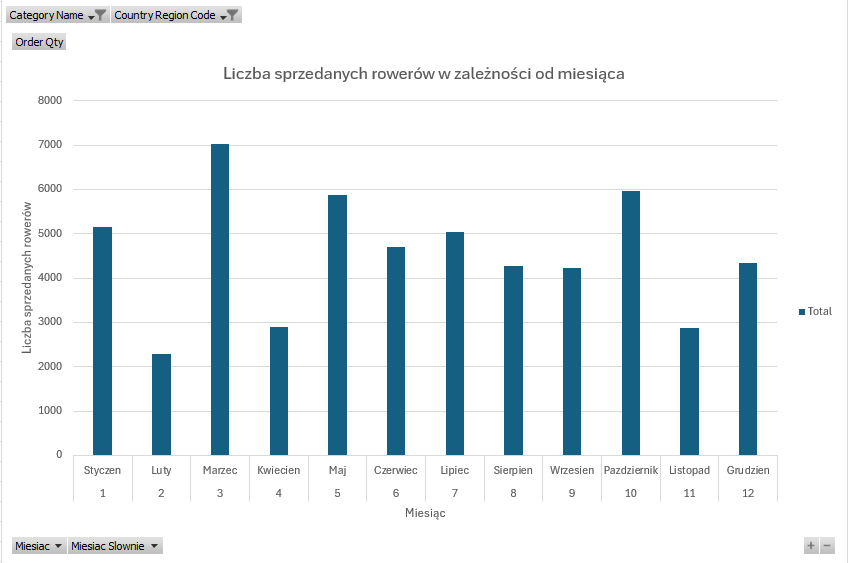
\includegraphics[width=0.6\textwidth]{images/bike_sales.png}
  \caption{Wykres}
\end{figure}

\subsubsection{Zniżka}

\begin{figure}[H]
  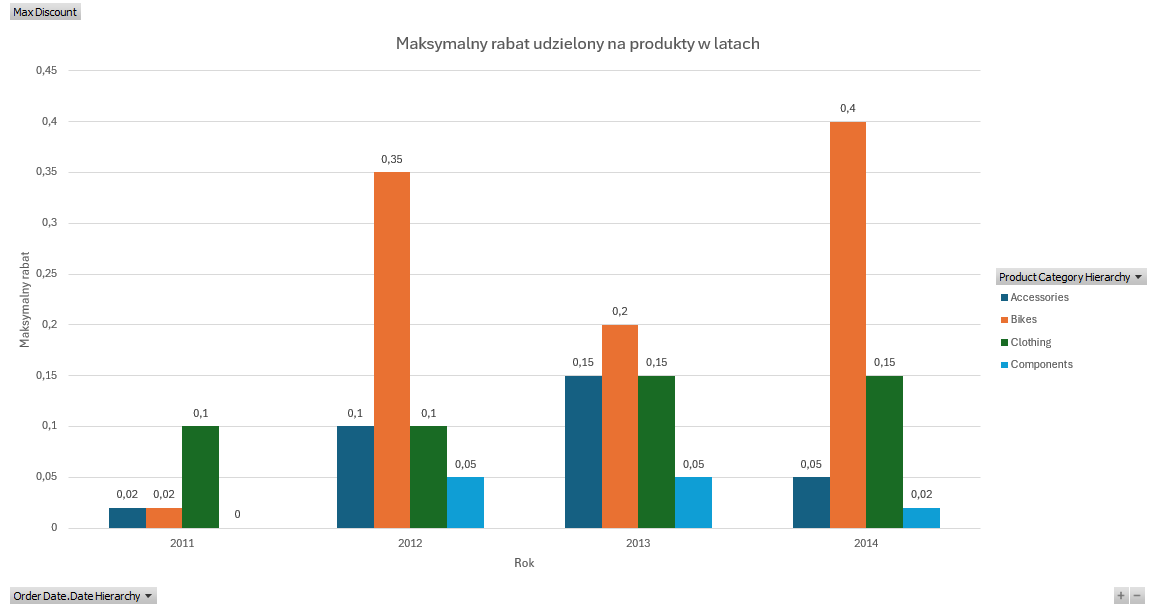
\includegraphics[width=0.6\textwidth]{images/max_discount.png}
  \caption{Wykres}
\end{figure}

\subsubsection{Sprzedawca}

\begin{figure}[H]
  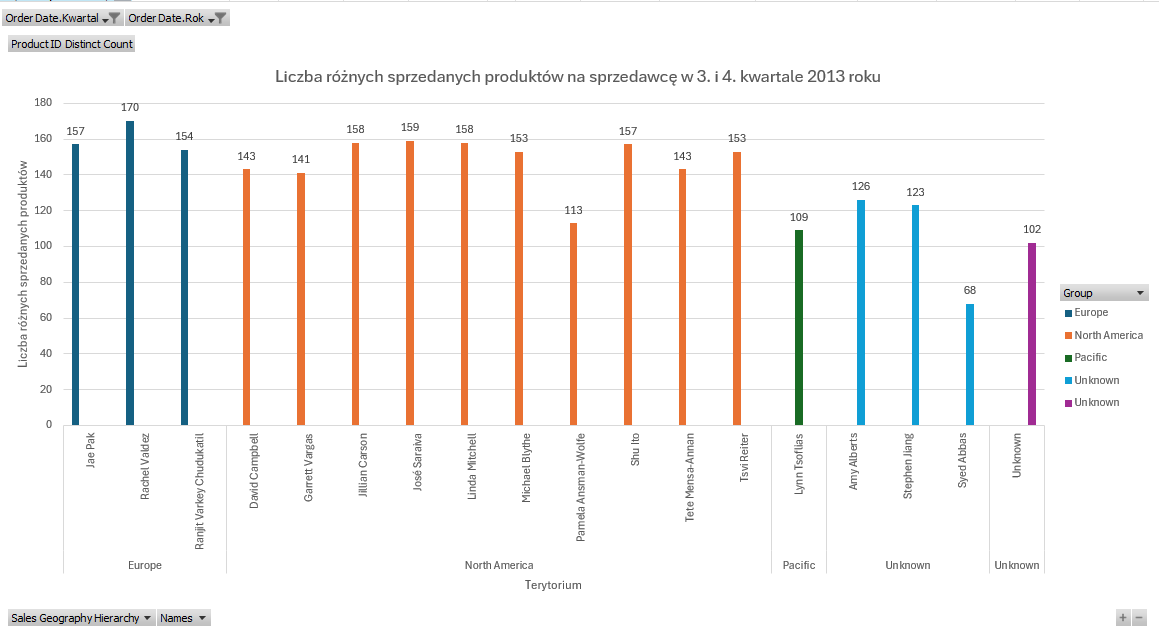
\includegraphics[width=0.6\textwidth]{images/sales_salesperson.png}
  \caption{Wykres}
\end{figure}

\section{Zad. 3. Miary kalkulowane}

W zakładce Calculations dodać dwie miary kalkulowane (ang. calculated members):\begin{itemize}
  \item średnią liczbę zamówionych towarów na zamówienie
  \item średnią ważoną liczbę towarów na zamówienie. Jako wagę należy wybrać cenę danego produktu.
\end{itemize}
Wskazówka: w celu utworzenia wyżej wymienionej średniej ważonej można posłużyć się nową
kolumną zdefiniowaną w widoku źródła danych (lub w tabeli). Kolumna ta powinna definiować
miarę pomocniczą, która pozwoli uzyskać fragment wyrażenia odpowiadającego średniej
ważonej.

\begin{figure}[H]
  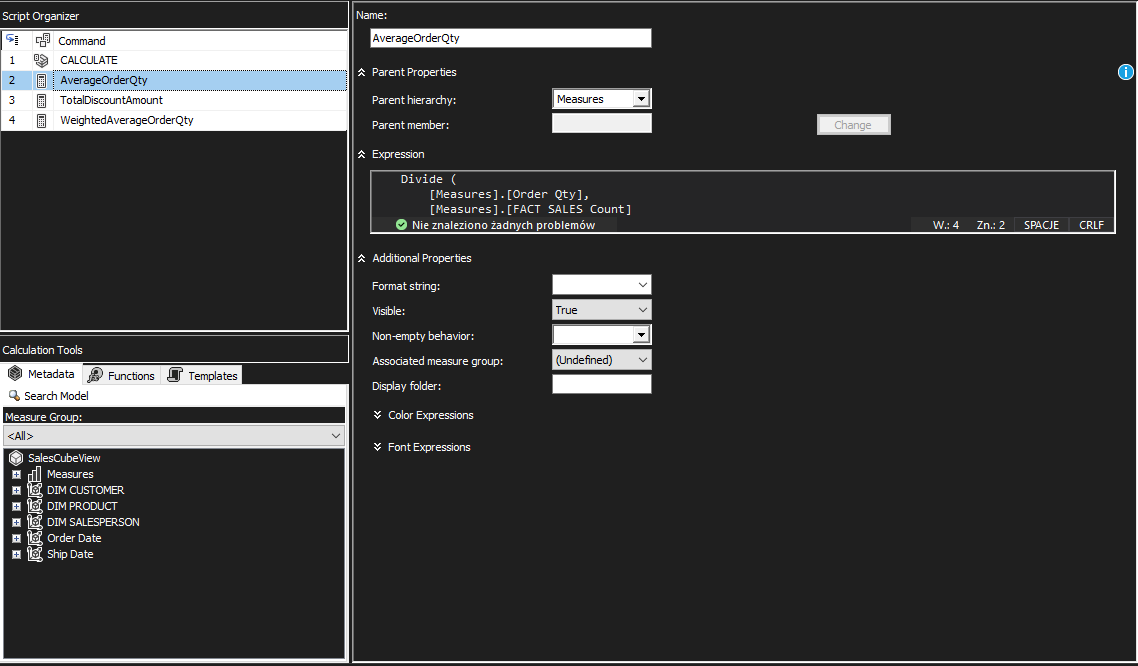
\includegraphics[width=0.6\textwidth]{images/3_calculations_1.png}
  \caption{Sposób obliczania miary ze zwykłą średnią}
\end{figure}

Do obliczenia średniej ważonej należało dodać miarę obliczającą sumę ceny jednostkowej i drugą miarę, będącą iloczynem ceny jednostkowej i liczby zamówionego produktu (LineTotal prawie to spełniał, ale miał w sobie czasem zniżkę).

\begin{figure}[H]
  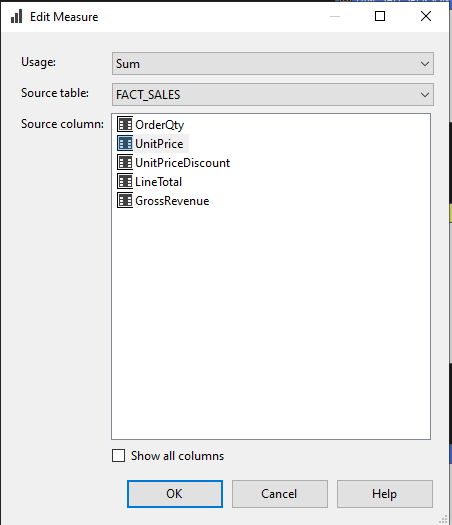
\includegraphics[width=0.6\textwidth]{images/3_sum_unit_price.png}
  \caption{Sposób obliczania miary z sumą ceny jednostkowej}
\end{figure}

\begin{figure}[H]
  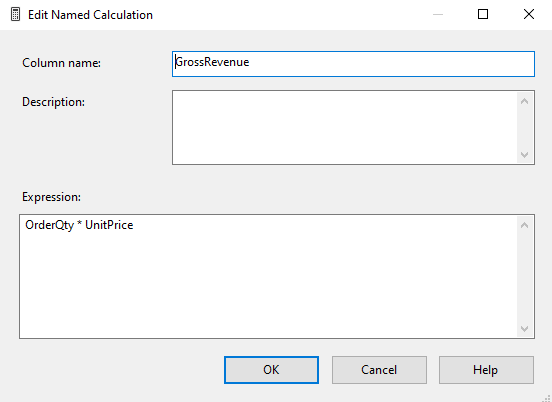
\includegraphics[width=0.6\textwidth]{images/3_gross_revenue.png}
  \caption{Sposób obliczania miary zysku brutto}
\end{figure}

\begin{figure}[H]
  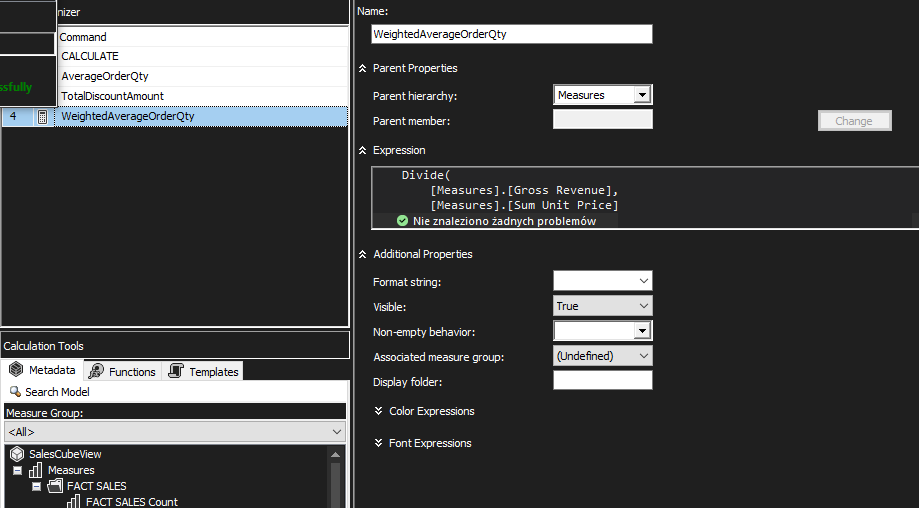
\includegraphics[width=0.6\textwidth]{images/3_calculations_2.png}
  \caption{Sposób obliczania miary średniej ważonej}
\end{figure}

\begin{figure}[H]
  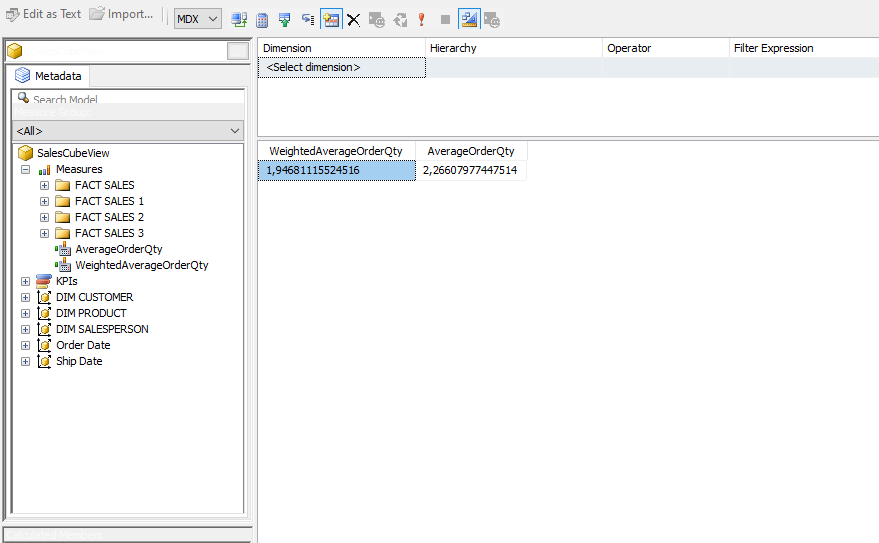
\includegraphics[width=0.6\textwidth]{images/3_result.png}
  \caption{Wynik średnich dla całego zbioru danych}
\end{figure}

\section{Zad. 4. Partycje}

Podzielić zawartość kostki na partycje (zakładka Partitions). Każda partycja powinna
odzwierciedlać jeden rok. Istnieją dwa podstawowe sposoby podziału partycjonowania kostek:
\begin{itemize}
  \item dane do zasilania poszczególnych partycji znajdują się w osobnych tabelach
  \item dane do zasilania poszczególnych partycji znajdują się w tej samej tabeli, zaś każda z partycji ma przypisanie zapytanie SQL, którego wynik służy do jej zasilenia.
\end{itemize}
Proszę przygotować partycje na dwa sposoby i znaleźć uzasadnienie dla każdej opcji.

\subsection{Sposób pierwszy}

Wymaga to stworzenia 4 nowych tabeli o schemacie identycznym do FACT\_SALES i wypełnienie ich odpowiednimi danymi.

\begin{lstlisting}[caption={Tworzenie i wypełnianie tabeli DIM\_TIME.}, label=lst:zad2_dim_time]
CREATE TABLE Kubs.FACT_SALES_2011 (
  ProductID INT FOREIGN KEY REFERENCES Kubs.DIM_PRODUCT(ProductID),
    CustomerID INT FOREIGN KEY REFERENCES Kubs.DIM_CUSTOMER(CustomerID),
    SalesPersonID INT FOREIGN KEY REFERENCES Kubs.DIM_SALESPERSON(SalesPersonID),
    OrderDate INT NOT NULL,
    ShipDate INT NULL,
    OrderQty SMALLINT NOT NULL,
    UnitPrice MONEY NOT NULL,
    UnitPriceDiscount DECIMAL(8, 4) NOT NULL,
    LineTotal DECIMAL(19, 4) NOT NULL
);

CREATE TABLE Kubs.FACT_SALES_2012 (
  ProductID INT FOREIGN KEY REFERENCES Kubs.DIM_PRODUCT(ProductID),
    CustomerID INT FOREIGN KEY REFERENCES Kubs.DIM_CUSTOMER(CustomerID),
    SalesPersonID INT FOREIGN KEY REFERENCES Kubs.DIM_SALESPERSON(SalesPersonID),
    OrderDate INT NOT NULL,
    ShipDate INT NULL,
    OrderQty SMALLINT NOT NULL,
    UnitPrice MONEY NOT NULL,
    UnitPriceDiscount DECIMAL(8, 4) NOT NULL,
    LineTotal DECIMAL(19, 4) NOT NULL
);

CREATE TABLE Kubs.FACT_SALES_2013 (
  ProductID INT FOREIGN KEY REFERENCES Kubs.DIM_PRODUCT(ProductID),
    CustomerID INT FOREIGN KEY REFERENCES Kubs.DIM_CUSTOMER(CustomerID),
    SalesPersonID INT FOREIGN KEY REFERENCES Kubs.DIM_SALESPERSON(SalesPersonID),
    OrderDate INT NOT NULL,
    ShipDate INT NULL,
    OrderQty SMALLINT NOT NULL,
    UnitPrice MONEY NOT NULL,
    UnitPriceDiscount DECIMAL(8, 4) NOT NULL,
    LineTotal DECIMAL(19, 4) NOT NULL
);

CREATE TABLE Kubs.FACT_SALES_2014 (
  ProductID INT FOREIGN KEY REFERENCES Kubs.DIM_PRODUCT(ProductID),
    CustomerID INT FOREIGN KEY REFERENCES Kubs.DIM_CUSTOMER(CustomerID),
    SalesPersonID INT FOREIGN KEY REFERENCES Kubs.DIM_SALESPERSON(SalesPersonID),
    OrderDate INT NOT NULL,
    ShipDate INT NULL,
    OrderQty SMALLINT NOT NULL,
    UnitPrice MONEY NOT NULL,
    UnitPriceDiscount DECIMAL(8, 4) NOT NULL,
    LineTotal DECIMAL(19, 4) NOT NULL
);

with Sales1 AS (
  SELECT 
    Kubs.FACT_SALES.ProductID,
    Kubs.FACT_SALES.CustomerID,
    Kubs.FACT_SALES.SalesPersonID,
    Kubs.FACT_SALES.OrderDate,
    Kubs.FACT_SALES.ShipDate,
    Kubs.FACT_SALES.OrderQty,
    Kubs.FACT_SALES.UnitPrice,
    Kubs.FACT_SALES.UnitPriceDiscount,
    Kubs.FACT_SALES.LineTotal
  FROM Kubs.FACT_SALES
  WHERE OrderDate >= 20110101 AND OrderDate < 20120000
)
INSERT INTO Kubs.FACT_SALES_2011

SELECT * FROM Sales1;

with Sales2 AS (
  SELECT 
    Kubs.FACT_SALES.ProductID,
    Kubs.FACT_SALES.CustomerID,
    Kubs.FACT_SALES.SalesPersonID,
    Kubs.FACT_SALES.OrderDate,
    Kubs.FACT_SALES.ShipDate,
    Kubs.FACT_SALES.OrderQty,
    Kubs.FACT_SALES.UnitPrice,
    Kubs.FACT_SALES.UnitPriceDiscount,
    Kubs.FACT_SALES.LineTotal
  FROM Kubs.FACT_SALES
  WHERE OrderDate >= 20120101 AND OrderDate < 20130000
)
INSERT INTO Kubs.FACT_SALES_2012

SELECT * FROM Sales2;

with Sales3 AS (
  SELECT 
    Kubs.FACT_SALES.ProductID,
    Kubs.FACT_SALES.CustomerID,
    Kubs.FACT_SALES.SalesPersonID,
    Kubs.FACT_SALES.OrderDate,
    Kubs.FACT_SALES.ShipDate,
    Kubs.FACT_SALES.OrderQty,
    Kubs.FACT_SALES.UnitPrice,
    Kubs.FACT_SALES.UnitPriceDiscount,
    Kubs.FACT_SALES.LineTotal
  FROM Kubs.FACT_SALES
  WHERE OrderDate >= 20130101 AND OrderDate < 20140000
)
INSERT INTO Kubs.FACT_SALES_2013

SELECT * FROM Sales3;

with Sales4 AS (
  SELECT 
    Kubs.FACT_SALES.ProductID,
    Kubs.FACT_SALES.CustomerID,
    Kubs.FACT_SALES.SalesPersonID,
    Kubs.FACT_SALES.OrderDate,
    Kubs.FACT_SALES.ShipDate,
    Kubs.FACT_SALES.OrderQty,
    Kubs.FACT_SALES.UnitPrice,
    Kubs.FACT_SALES.UnitPriceDiscount,
    Kubs.FACT_SALES.LineTotal
  FROM Kubs.FACT_SALES
  WHERE OrderDate >= 20140101
)
INSERT INTO Kubs.FACT_SALES_2014
\end{lstlisting}

Następnie należało dodać każdą z tabel do projektu, a potem do partycji w kostce.

\begin{figure}[H]
  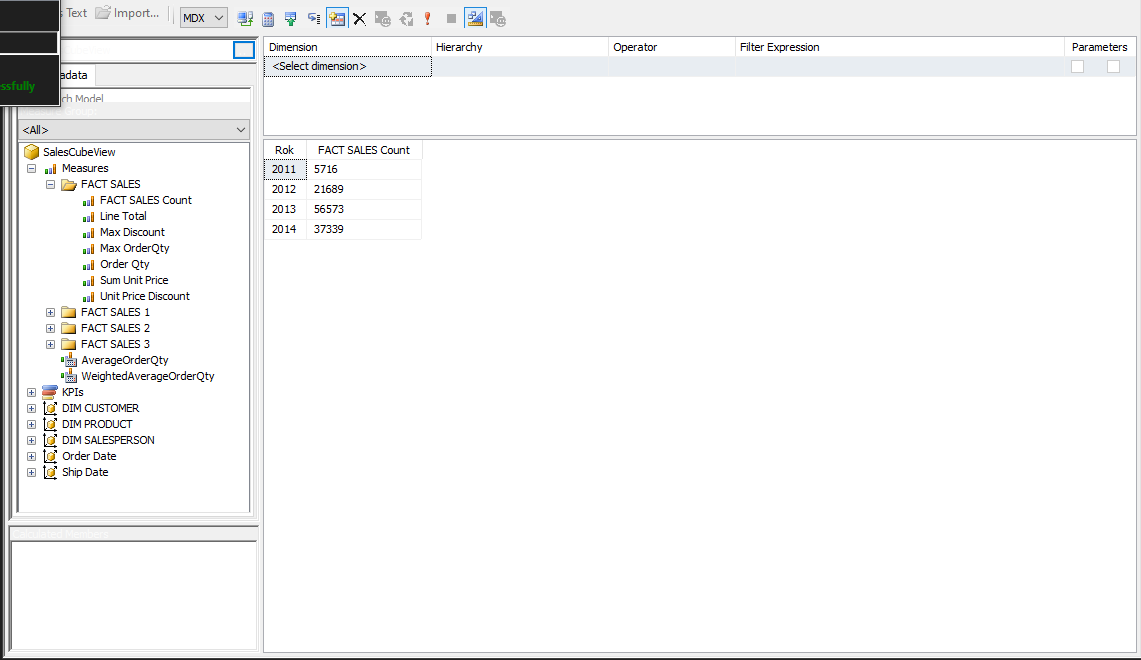
\includegraphics[width=0.6\textwidth]{images/4a.png}
  \caption{Dodane partycje}
\end{figure}

\begin{figure}[H]
  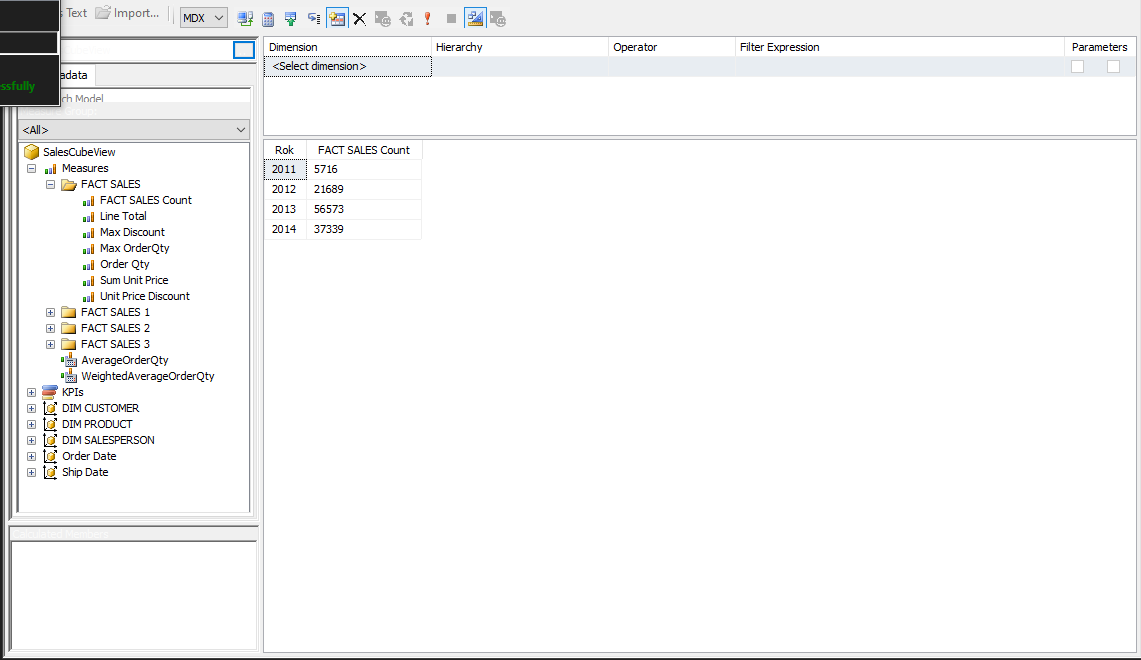
\includegraphics[width=0.6\textwidth]{images/4a_result.png}
  \caption{Wynik}
\end{figure}

\subsection{Sposób drugi}

To podejście było teoretycznie prostsze - wystarczyło zmienić kod SQL w nowo dodawanych partycjach

\begin{figure}[H]
  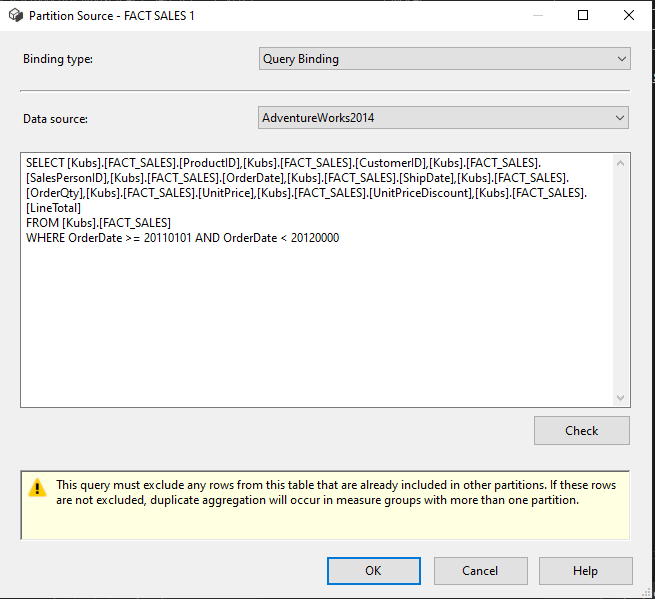
\includegraphics[width=0.6\textwidth]{images/4b_source.png}
  \caption{Zmieniony kod SQL w partycji - dodana klauzula WHERE ograniczająca daty}
\end{figure}

\begin{figure}[H]
  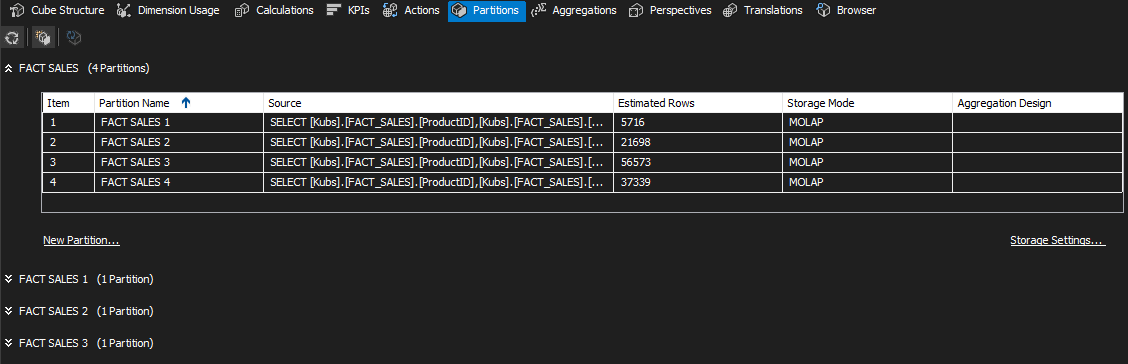
\includegraphics[width=0.6\textwidth]{images/4b.png}
  \caption{Dodane partycje}
\end{figure}

\begin{figure}[H]
  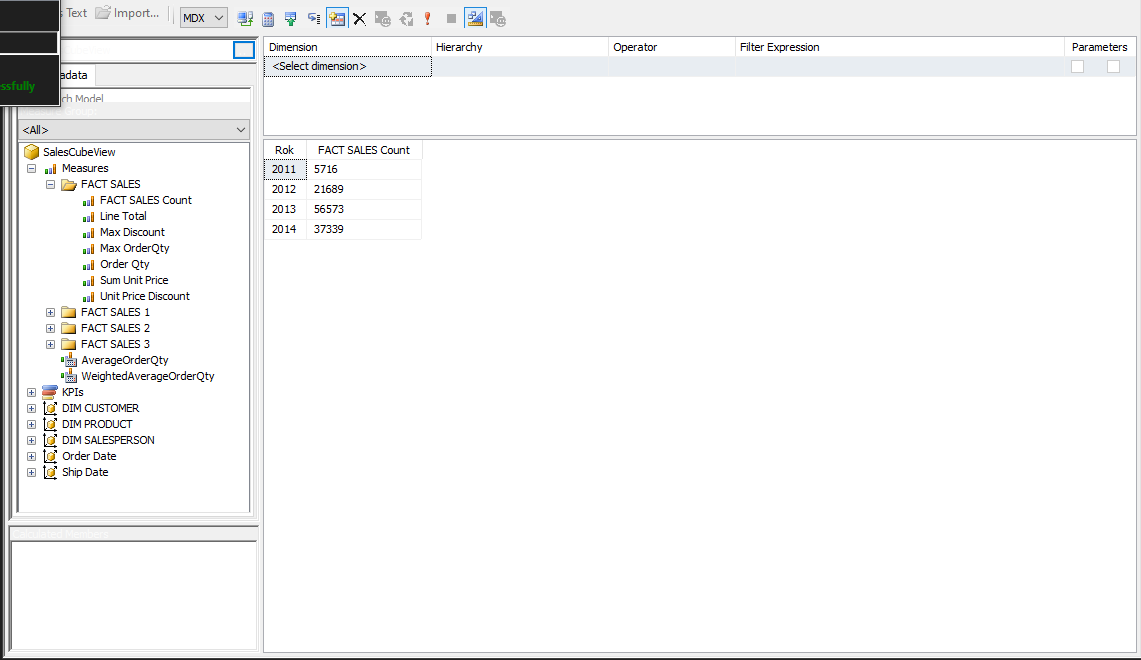
\includegraphics[width=0.6\textwidth]{images/4a_result.png}
  \caption{Wynik}
\end{figure}

\section{Zad. 5. * Definiowanie KPI}
\section{Wnioski}

\section{Wnioski}

\printbibliography

\end{document}